\documentclass{standalone}
\usepackage{tikz}
\usetikzlibrary{patterns, positioning}
\usepackage[sfdefault]{ClearSans} %% option 'sfdefault' activates Clear Sans as the default text font
\usepackage[T1]{fontenc}

\begin{document}
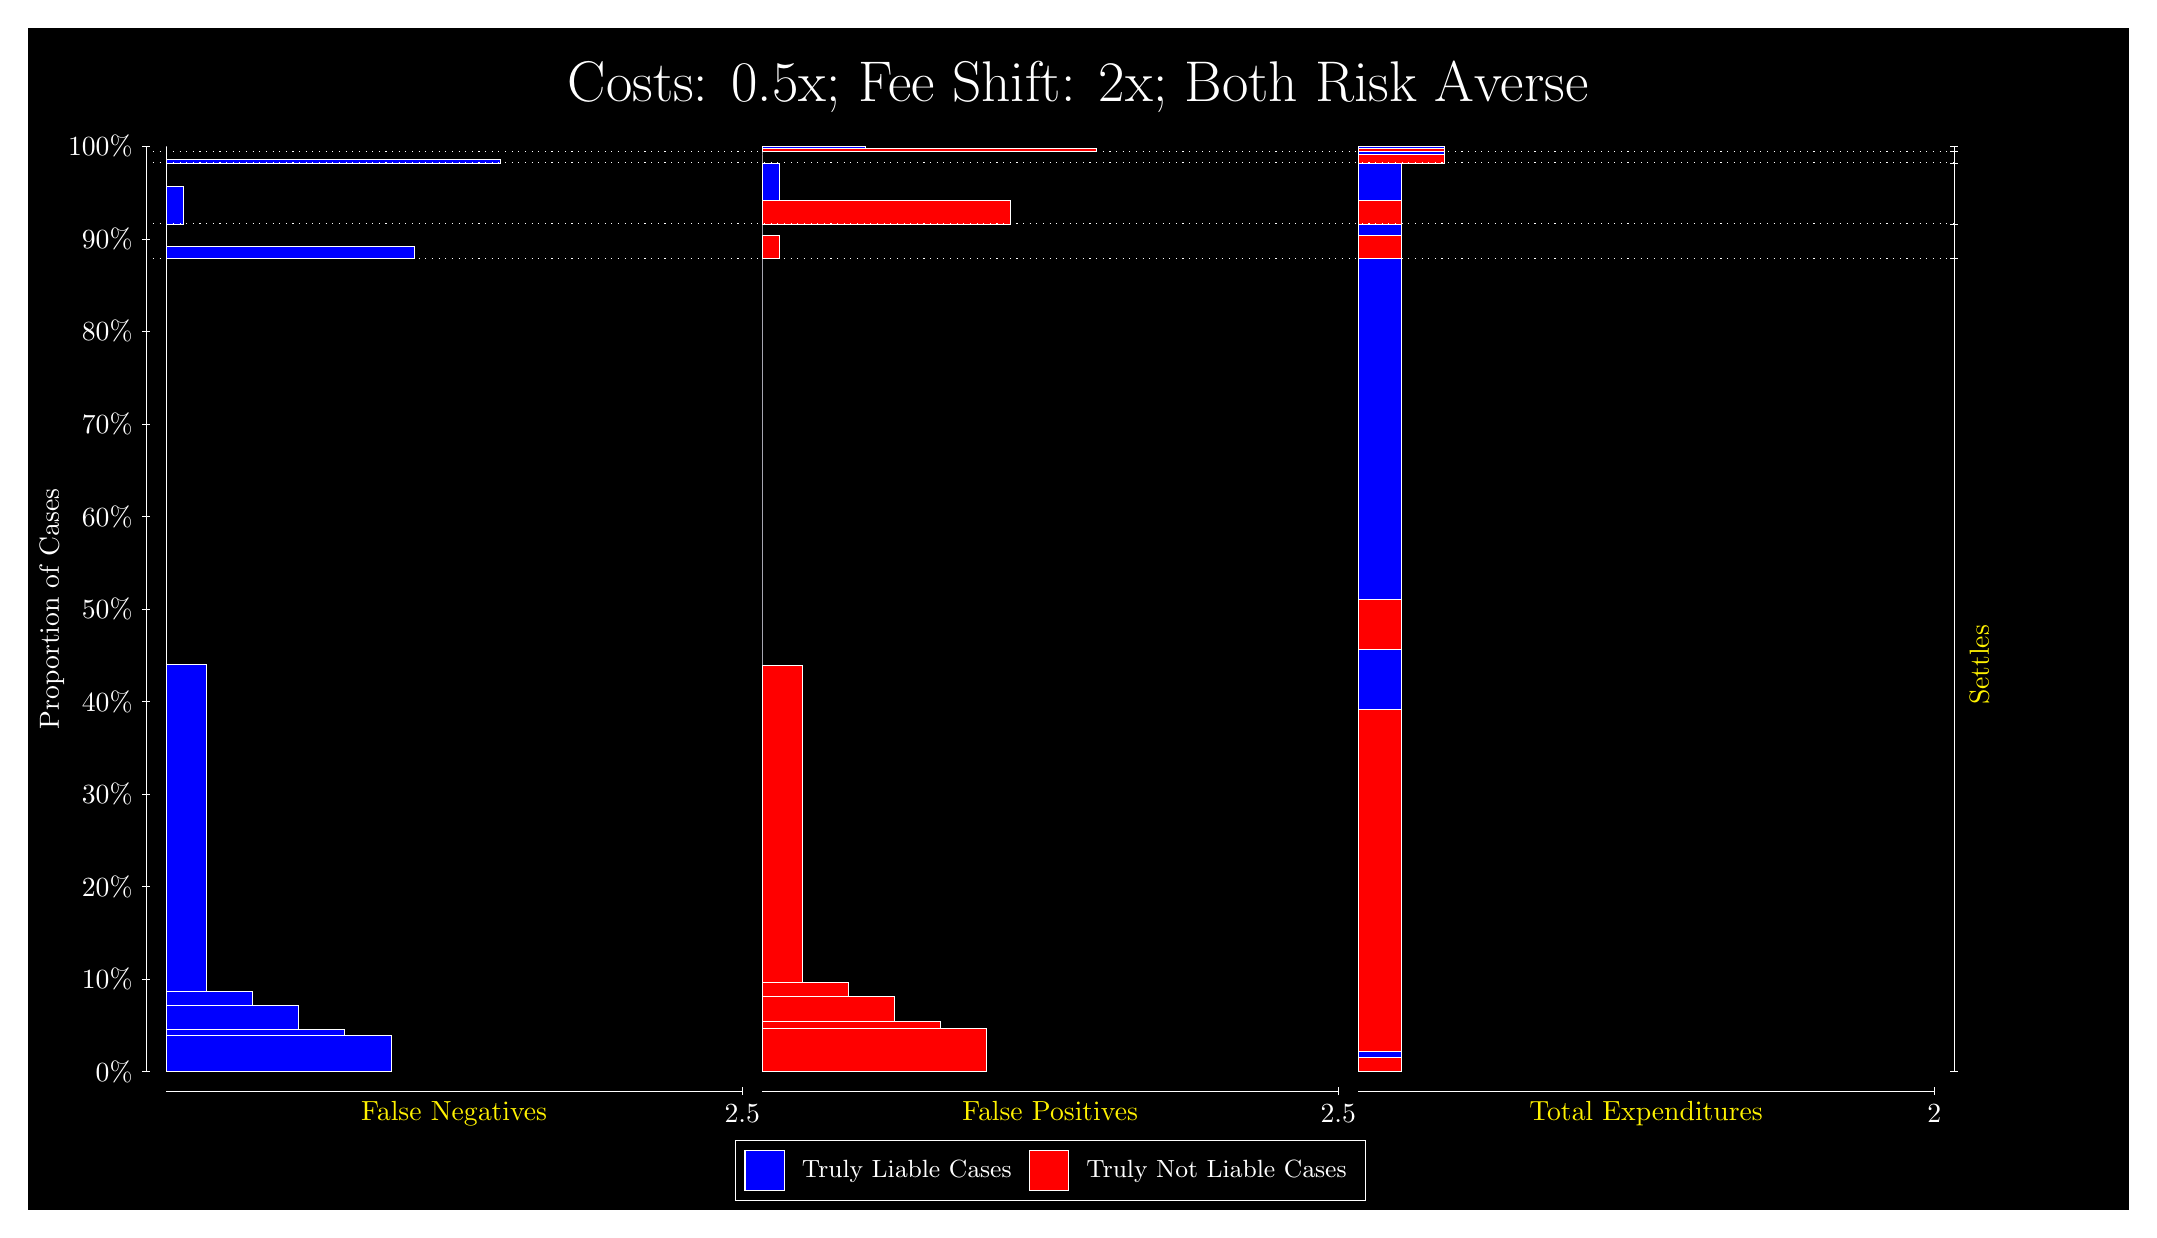
\begin{tikzpicture}
\draw[fill=black] (0,0) rectangle (26.667,15);
\draw[text=white] (0,13.5) rectangle (26.667,15) node[midway] {\huge Costs: 0.5x; Fee Shift: 2x; Both Risk Averse};
\draw[white, very thin] (1.5,1.75) -- (1.5,13.5);
\node[rotate=90, text=white, anchor=center] at (0.3, 7.625) {Proportion of Cases};
\draw[white, very thin] (1.45,1.75) -- (1.55,1.75);
\node[text=white, anchor=east] at (1.45, 1.75) {0\%};
\draw[white, very thin] (1.45,2.925) -- (1.55,2.925);
\node[text=white, anchor=east] at (1.45, 2.925) {10\%};
\draw[white, very thin] (1.45,4.1) -- (1.55,4.1);
\node[text=white, anchor=east] at (1.45, 4.1) {20\%};
\draw[white, very thin] (1.45,5.275) -- (1.55,5.275);
\node[text=white, anchor=east] at (1.45, 5.275) {30\%};
\draw[white, very thin] (1.45,6.45) -- (1.55,6.45);
\node[text=white, anchor=east] at (1.45, 6.45) {40\%};
\draw[white, very thin] (1.45,7.625) -- (1.55,7.625);
\node[text=white, anchor=east] at (1.45, 7.625) {50\%};
\draw[white, very thin] (1.45,8.8) -- (1.55,8.8);
\node[text=white, anchor=east] at (1.45, 8.8) {60\%};
\draw[white, very thin] (1.45,9.975) -- (1.55,9.975);
\node[text=white, anchor=east] at (1.45, 9.975) {70\%};
\draw[white, very thin] (1.45,11.15) -- (1.55,11.15);
\node[text=white, anchor=east] at (1.45, 11.15) {80\%};
\draw[white, very thin] (1.45,12.325) -- (1.55,12.325);
\node[text=white, anchor=east] at (1.45, 12.325) {90\%};
\draw[white, very thin] (1.45,13.5) -- (1.55,13.5);
\node[text=white, anchor=east] at (1.45, 13.5) {100\%};

\draw[white, very thin] (24.457,1.75) -- (24.457,13.5);
\draw[white, very thin] (24.407,1.75) -- (24.507,1.75);
\node[anchor=west] at (24.407, 1.75) {};
\draw[white, very thin] (24.407,12.079) -- (24.507,12.079);
\node[anchor=west] at (24.407, 12.079) {};
\draw[white, very thin] (24.407,12.516) -- (24.507,12.516);
\node[anchor=west] at (24.407, 12.516) {};
\draw[white, very thin] (24.407,13.29) -- (24.507,13.29);
\node[anchor=west] at (24.407, 13.29) {};
\draw[white, very thin] (24.407,13.438) -- (24.507,13.438);
\node[anchor=west] at (24.407, 13.438) {};
\draw[white, very thin] (24.407,13.5) -- (24.507,13.5);
\node[anchor=west] at (24.407, 13.5) {};

\draw[white, very thin, fill=blue] (1.75,1.75) rectangle (4.6044,2.2093);
\draw[white, very thin, fill=blue] (1.75,2.2093) rectangle (4.0188,2.2879);
\draw[white, very thin, fill=blue] (1.75,2.2879) rectangle (3.4333,2.59);
\draw[white, very thin, fill=blue] (1.75,2.59) rectangle (2.8478,2.7683);
\draw[white, very thin, fill=blue] (1.75,2.7683) rectangle (2.2623,6.9261);
\draw[white, very thin, fill=red] (1.75,6.9261) rectangle (1.75,12.079);
\draw[white, very thin, fill=blue] (1.75,12.079) rectangle (4.8971,12.228);
\draw[white, very thin, fill=red] (1.75,12.228) rectangle (1.75,12.516);
\draw[white, very thin, fill=blue] (1.75,12.516) rectangle (1.9696,12.991);
\draw[white, very thin, fill=red] (1.75,12.991) rectangle (1.75,13.29);
\draw[white, very thin, fill=blue] (1.75,13.29) rectangle (5.9949,13.334);
\draw[white, very thin, fill=red] (1.75,13.334) rectangle (1.75,13.438);
\draw[white, very thin, fill=red] (1.75,13.438) rectangle (1.75,13.469);
\draw[white, very thin, fill=blue] (1.75,13.469) rectangle (1.75,13.5);
\draw[white, very thin, fill=red] (9.3189,1.75) rectangle (12.173,2.3036);
\draw[white, very thin, fill=red] (9.3189,2.3036) rectangle (11.588,2.3822);
\draw[white, very thin, fill=red] (9.3189,2.3822) rectangle (11.002,2.7069);
\draw[white, very thin, fill=red] (9.3189,2.7069) rectangle (10.417,2.8852);
\draw[white, very thin, fill=red] (9.3189,2.8852) rectangle (9.8312,6.9034);
\draw[white, very thin, fill=blue] (9.3189,6.9034) rectangle (9.3189,12.079);
\draw[white, very thin, fill=red] (9.3189,12.079) rectangle (9.5384,12.367);
\draw[white, very thin, fill=blue] (9.3189,12.367) rectangle (9.3189,12.516);
\draw[white, very thin, fill=red] (9.3189,12.516) rectangle (12.466,12.815);
\draw[white, very thin, fill=blue] (9.3189,12.815) rectangle (9.5384,13.29);
\draw[white, very thin, fill=red] (9.3189,13.29) rectangle (9.3189,13.394);
\draw[white, very thin, fill=blue] (9.3189,13.394) rectangle (9.3189,13.438);
\draw[white, very thin, fill=red] (9.3189,13.438) rectangle (13.564,13.469);
\draw[white, very thin, fill=blue] (9.3189,13.469) rectangle (10.636,13.5);
\draw[white, very thin, fill=red] (16.888,1.75) rectangle (17.437,1.9283);
\draw[white, very thin, fill=blue] (16.888,1.9283) rectangle (17.437,2.0069);
\draw[white, very thin, fill=red] (16.888,2.0069) rectangle (17.437,6.3498);
\draw[white, very thin, fill=blue] (16.888,6.3498) rectangle (17.437,7.1111);
\draw[white, very thin, fill=red] (16.888,7.1111) rectangle (17.437,7.7433);
\draw[white, very thin, fill=blue] (16.888,7.7433) rectangle (17.437,12.079);
\draw[white, very thin, fill=red] (16.888,12.079) rectangle (17.437,12.367);
\draw[white, very thin, fill=blue] (16.888,12.367) rectangle (17.437,12.516);
\draw[white, very thin, fill=red] (16.888,12.516) rectangle (17.437,12.815);
\draw[white, very thin, fill=blue] (16.888,12.815) rectangle (17.437,13.29);
\draw[white, very thin, fill=red] (16.888,13.29) rectangle (17.986,13.394);
\draw[white, very thin, fill=blue] (16.888,13.394) rectangle (17.986,13.438);
\draw[white, very thin, fill=red] (16.888,13.438) rectangle (17.986,13.469);
\draw[white, very thin, fill=blue] (16.888,13.469) rectangle (17.986,13.5);
\draw[white, dotted] (1.5,12.079) -- (24.457,12.079);
\draw[white, dotted] (1.5,12.516) -- (24.457,12.516);
\draw[white, dotted] (1.5,13.29) -- (24.457,13.29);
\draw[white, dotted] (1.5,13.438) -- (24.457,13.438);
\draw[white, very thin] (1.75,1.5) -- (9.0689,1.5);
\node[text=yellow, anchor=north] at (5.4094, 1.5) {False Negatives};
\draw[white, very thin] (9.0689,1.45) -- (9.0689,1.55);
\node[text=white, anchor=north] at (9.0689, 1.45) {2.5};

\draw[white, very thin] (9.3189,1.5) -- (16.638,1.5);
\node[text=yellow, anchor=north] at (12.978, 1.5) {False Positives};
\draw[white, very thin] (16.638,1.45) -- (16.638,1.55);
\node[text=white, anchor=north] at (16.638, 1.45) {2.5};

\draw[white, very thin] (16.888,1.5) -- (24.207,1.5);
\node[text=yellow, anchor=north] at (20.547, 1.5) {Total Expenditures};
\draw[white, very thin] (24.207,1.45) -- (24.207,1.55);
\node[text=white, anchor=north] at (24.207, 1.45) {2};

\node[text=yellow, centered, rotate=90] at (24.777, 6.9147) {Settles};





\draw (12.978300999999998,1.5) node[draw=none] (baseCoordinate) {};
\begin{scope}[align=center]
        \matrix[scale=0.5, draw=white, below=0.5cm of baseCoordinate, nodes={draw}, column sep=0.1cm]{
            \node[rectangle, draw, minimum width=0.5cm, minimum height=0.5cm, fill=blue] {}; &
            \node[draw=none, font=\small, text=white] (B) {Truly Liable Cases}; &
            \node[rectangle, draw, minimum width=0.5cm, minimum height=0.5cm, fill=red] {}; &
            \node[draw=none, font=\small, text=white] (B) {Truly Not Liable Cases}; \\
            };
\end{scope}

\end{tikzpicture}
\end{document}